
\newcommand{\OperatorSpace}[5]{
				%\draw[rounded corners = 15pt,dashed] (#1-#4,#2-#5) rectangle (#1+#4,#2+#5);
		\fill[fill=green,opacity=0.2] (#1,#2) circle (#3);
		\draw[draw = black,dashed](#1,#2) circle (#3);
		%\node at (#1,#2-#5+0.5) {$\mathcal{T}_{#6}$};
	}
\tikzset{cross/.style={cross out, draw=black, minimum size=2*(#1-\pgflinewidth), inner sep=0pt, outer sep=0pt},
	%default radius will be 1pt. 
	cross/.default={4pt}}
	
\begin{figure}[h!]
	\centering
		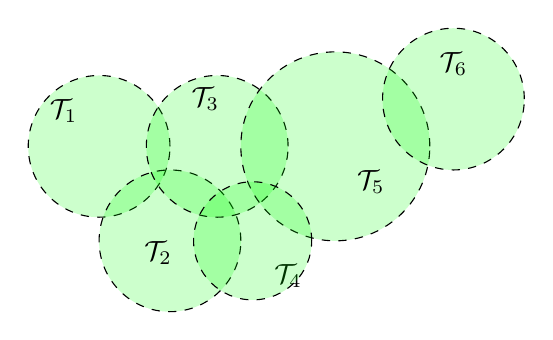
\begin{tikzpicture}[scale=0.3]
			\OperatorSpace{0}{0}{3}{5}{5}
			%\node at (-4.25,4.25){$S_1$};
			\node at (-1.5,1.5){$\mathcal{T}_1$};
			\OperatorSpace{3}{-4}{3}{5}{5}
			%\node at (-1.25,-8.25){$S_2$};
			\node at (2.5,-4.5){$\mathcal{T}_2$};
			%\node[red] at (2.5,3) (H13) {$H_{13}$};
			%\draw [->,red,line width = 0.75mm] (H13) -- (2.5,1.25);
			\OperatorSpace{5}{0}{3}{5}{6}
			%\node at (5-4.25,5.5){$S_3$};
			\node at (5-0.5,2){$\mathcal{T}_3$};
			%\node[red] at (6.5,3.5) (H35) {$H_{35}$};
			%\draw [->,red,line width = 0.75mm] (H35) -- (6.75,0.65);
			\OperatorSpace{10}{0}{4}{6}{7}
			
			\node at (8.5-0.5,-5.5){$\mathcal{T}_4$};
% 			\node[red] at (6.5,3.5) (H35) {$H_{35}$};
			%\draw [->,red,line width = 0.75mm] (H35) -- (6.75,0.65);
			\OperatorSpace{6.5}{-4}{2.5}{0}{0}
			
			%\node at (10+5.25,-6.5){$S_5$};
			\node at (10+1.5,-1.5){$\mathcal{T}_5$};
			\OperatorSpace{15}{2}{3}{5}{5}
			%\node at (15-4.25,5+3.25){$S_6$};
			\node at (15,3.5){$\mathcal{T}_6$};
			%\node[red] at (11,4.5) (H56) {$H_{56}$};
			%\draw [->,red,line width = 0.75mm] (H56) -- (12.5,2.75);

			
		\end{tikzpicture}
%		\setlength{\belowcaptionskip}{-2pt}
        \caption{Example UAM operating environment. Green circles correspond to the regions of vertihub controllers.}
	        \label{fig:RegionsOutline}
    \end{figure}